% Figure clh_lean_slice_map: the gradient G_f on a plane of the gauge slice: a grid near theta and lines across the slice.
% Illustrates CLH-1 (Section sec:homeo: injectivity and homeomorphism). Inputs: f-bar = (3,5,1,2,4), theta/pi = (0, 0.1, 0.7, 0.3, 0.8); the plane is theta + pi (s e_3 + t e_2).
% Source of the figure, typeset in the paper's own fonts (T1, Latin Modern, 11pt) at the paper's text
% width (6.5in), so \includegraphics does not rescale it. It adds no assertion.
% Every coordinate is read from numerical values computed by floating-point code that follows the
% paper's formulas (the pictures' Lean helper); the SHA-256 of each output line it comes from:
%   D55_s56_default 035d7fd57dede709bed81e049156117d422369f636ddbbc37fdc141dd2de46ed
%   D58_s58_default 3271f3d8c5227642ff92dc0916780ab6b202e9409c51985817f7195a22ff1be1
% Build: pdflatex <this file> && pdftocairo -svg <this file>.pdf <this file>.svg

\documentclass[11pt]{standalone}
\usepackage[T1]{fontenc}
\usepackage{lmodern}
\usepackage{amsmath,amssymb}
\usepackage{tikz}
\usetikzlibrary{arrows.meta,calc}

% the palette of the paper's other figures: blue solid for the first object, ochre dashed for the second
\definecolor{ink}{HTML}{233740}
\definecolor{muted}{HTML}{65757D}
\definecolor{pblue}{HTML}{0072B2}
\definecolor{qochre}{HTML}{B87827}

\tikzset{
  ax/.style={draw=muted, line width=0.5pt},
  axd/.style={draw=muted!70, line width=0.4pt, dash pattern=on 1.5pt off 2pt},
  tick/.style={draw=muted, line width=0.5pt},
  lab/.style={font=\footnotesize, inner sep=1.2pt, text=ink},
  labm/.style={font=\small, inner sep=1.2pt, text=ink},
  labw/.style={font=\footnotesize, inner sep=1pt, text=ink, fill=white, fill opacity=0.8, text opacity=1},
  labP/.style={font=\footnotesize, inner sep=1.2pt, text=pblue},
  labQ/.style={font=\footnotesize, inner sep=1.2pt, text=qochre},
  tk/.style={font=\footnotesize, inner sep=1pt, text=muted},
  panel/.style={font=\small, inner sep=0pt, text=ink},
  curveP/.style={pblue, line width=1.1pt, line cap=round, line join=round},
  thinP/.style={pblue, line width=0.8pt, line cap=round, line join=round},
  thinQ/.style={qochre, line width=0.8pt, dash pattern=on 3pt off 1.6pt, line cap=round, line join=round},
  curveQ/.style={qochre, line width=1.1pt, dash pattern=on 4pt off 1.6pt, line cap=round},
  fillP/.style={pblue, fill=pblue!8, line width=1.1pt, line join=round},
  dotI/.style={circle, draw=ink, fill=ink, line width=0.6pt, inner sep=0pt, minimum size=4.6pt},
  dotIs/.style={circle, draw=ink, fill=ink, line width=0.5pt, inner sep=0pt, minimum size=3.2pt},
  ringI/.style={circle, draw=ink, fill=white, line width=0.6pt, inner sep=0pt, minimum size=4.6pt},
  dotP/.style={circle, draw=pblue, fill=pblue, line width=0.6pt, inner sep=0pt, minimum size=4.6pt},
  dotQ/.style={circle, draw=qochre, fill=qochre, line width=0.6pt, inner sep=0pt, minimum size=4.6pt},
  dotQs/.style={circle, draw=qochre, fill=qochre, line width=0.5pt, inner sep=0pt, minimum size=3pt},
  ringQ/.style={circle, draw=qochre, fill=white, line width=0.6pt, inner sep=0pt, minimum size=4.6pt},
}

\begin{document}
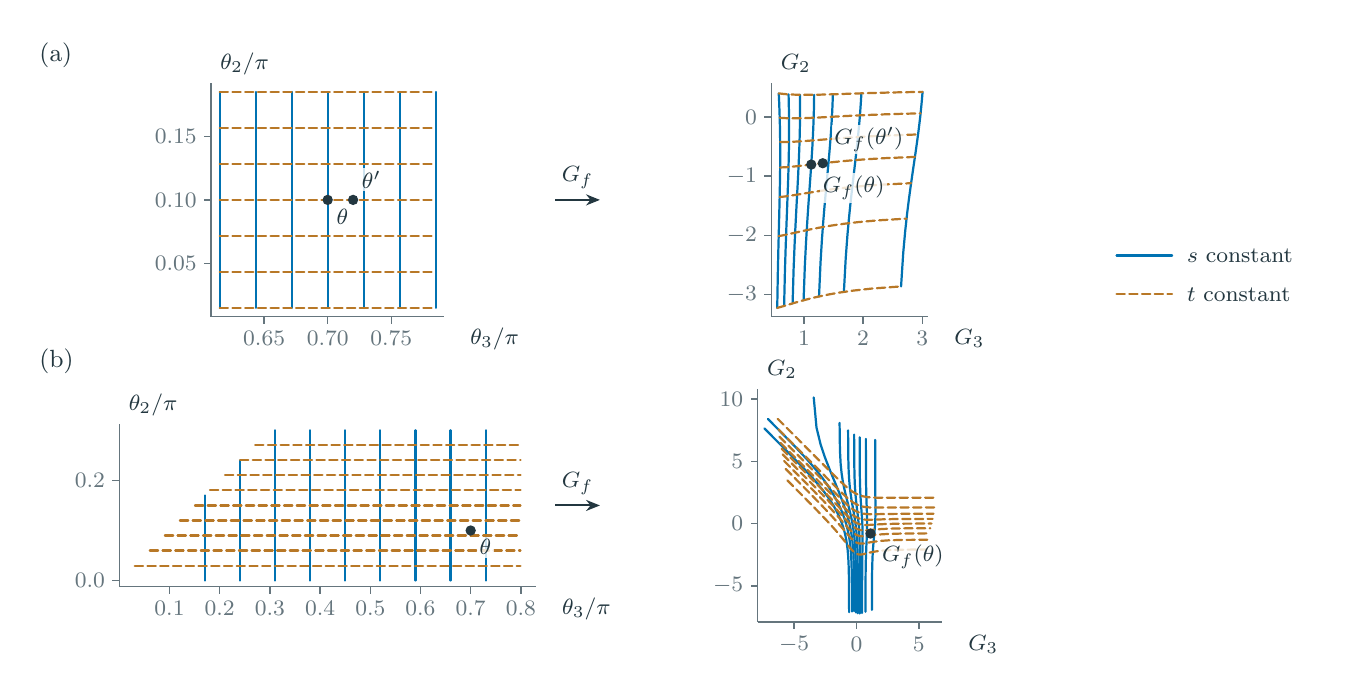
\begin{tikzpicture}[x=1bp,y=1bp]
\useasboundingbox (0bp,0bp) rectangle (468bp,232bp);
%box Ad 66 128 84 84 0.6082 0.7918 0.0082 0.1918
%box Ai 267.7472753 128 56.5054493 84 0.4512042834 3.103392742 -3.372895079 0.5698013027
\draw[ax] (66.00,128.00) -- (150.00,128.00); %line
\draw[ax] (66.00,128.00) -- (66.00,212.00); %line
\draw[tick] (85.12,128.00) -- (85.12,125.50); %tickx Ad 0.65
\node[tk] at (85.12,120.00) {$0.65$}; %num Ad-xt 0.65
\draw[tick] (108.00,128.00) -- (108.00,125.50); %tickx Ad 0.7
\node[tk] at (108.00,120.00) {$0.70$}; %num Ad-xt 0.7
\draw[tick] (130.88,128.00) -- (130.88,125.50); %tickx Ad 0.75
\node[tk] at (130.88,120.00) {$0.75$}; %num Ad-xt 0.75
\draw[tick] (66.00,147.12) -- (63.50,147.12); %ticky Ad 0.05
\node[tk, anchor=east] at (62.00,147.12) {$0.05$}; %num Ad-yt 0.05
\draw[tick] (66.00,170.00) -- (63.50,170.00); %ticky Ad 0.1
\node[tk, anchor=east] at (62.00,170.00) {$0.10$}; %num Ad-yt 0.1
\draw[tick] (66.00,192.88) -- (63.50,192.88); %ticky Ad 0.15
\node[tk, anchor=east] at (62.00,192.88) {$0.15$}; %num Ad-yt 0.15
\draw[ax] (267.75,128.00) -- (324.25,128.00); %line
\draw[ax] (267.75,128.00) -- (267.75,212.00); %line
\draw[tick] (279.44,128.00) -- (279.44,125.50); %tickx Ai 1
\node[tk] at (279.44,120.00) {$1$}; %num Ai-xt 1
\draw[tick] (300.74,128.00) -- (300.74,125.50); %tickx Ai 2
\node[tk] at (300.74,120.00) {$2$}; %num Ai-xt 2
\draw[tick] (322.05,128.00) -- (322.05,125.50); %tickx Ai 3
\node[tk] at (322.05,120.00) {$3$}; %num Ai-xt 3
\draw[tick] (267.75,135.94) -- (265.25,135.94); %ticky Ai -3
\node[tk, anchor=east] at (263.75,135.94) {${-}3$}; %num Ai-yt -3
\draw[tick] (267.75,157.25) -- (265.25,157.25); %ticky Ai -2
\node[tk, anchor=east] at (263.75,157.25) {${-}2$}; %num Ai-yt -2
\draw[tick] (267.75,178.56) -- (265.25,178.56); %ticky Ai -1
\node[tk, anchor=east] at (263.75,178.56) {${-}1$}; %num Ai-yt -1
\draw[tick] (267.75,199.86) -- (265.25,199.86); %ticky Ai 0
\node[tk, anchor=east] at (263.75,199.86) {$0$}; %num Ai-yt 0
\draw[thinP] (69.11,131.11) -- (69.11,135.97) -- (69.11,140.83) -- (69.11,145.69) -- (69.11,150.56) -- (69.11,155.42) -- (69.11,160.28) -- (69.11,165.14) -- (69.11,170.00) -- (69.11,174.86) -- (69.11,179.72) -- (69.11,184.58) -- (69.11,189.44) -- (69.11,194.31) -- (69.11,199.17) -- (69.11,204.03) -- (69.11,208.89); %poly Ad/l0
\draw[thinP] (269.84,131.11) -- (270.06,143.73) -- (270.25,152.34) -- (270.42,159.05) -- (270.56,164.64) -- (270.68,169.51) -- (270.77,173.89) -- (270.84,177.91) -- (270.89,181.67) -- (270.91,185.23) -- (270.91,188.66) -- (270.88,191.98) -- (270.83,195.25) -- (270.76,198.48) -- (270.66,201.72) -- (270.54,204.99) -- (270.39,208.34); %poly Ai/l0
\draw[thinP] (82.07,131.11) -- (82.07,135.97) -- (82.07,140.83) -- (82.07,145.69) -- (82.07,150.56) -- (82.07,155.42) -- (82.07,160.28) -- (82.07,165.14) -- (82.07,170.00) -- (82.07,174.86) -- (82.07,179.72) -- (82.07,184.58) -- (82.07,189.44) -- (82.07,194.31) -- (82.07,199.17) -- (82.07,204.03) -- (82.07,208.89); %poly Ad/l1
\draw[thinP] (272.32,131.82) -- (272.61,144.38) -- (272.88,152.91) -- (273.11,159.55) -- (273.32,165.07) -- (273.50,169.88) -- (273.66,174.20) -- (273.80,178.15) -- (273.91,181.84) -- (273.99,185.34) -- (274.05,188.70) -- (274.09,191.97) -- (274.10,195.17) -- (274.09,198.34) -- (274.06,201.51) -- (274.00,204.72) -- (273.92,208.00); %poly Ai/l1
\draw[thinP] (95.04,131.11) -- (95.04,135.97) -- (95.04,140.83) -- (95.04,145.69) -- (95.04,150.56) -- (95.04,155.42) -- (95.04,160.28) -- (95.04,165.14) -- (95.04,170.00) -- (95.04,174.86) -- (95.04,179.72) -- (95.04,184.58) -- (95.04,189.44) -- (95.04,194.31) -- (95.04,199.17) -- (95.04,204.03) -- (95.04,208.89); %poly Ad/l2
\draw[thinP] (275.38,132.73) -- (275.74,145.21) -- (276.08,153.67) -- (276.39,160.23) -- (276.67,165.69) -- (276.92,170.43) -- (277.15,174.68) -- (277.35,178.56) -- (277.52,182.19) -- (277.67,185.63) -- (277.80,188.92) -- (277.90,192.12) -- (277.98,195.26) -- (278.03,198.36) -- (278.06,201.48) -- (278.07,204.62) -- (278.05,207.84); %poly Ai/l2
\draw[thinP] (108.00,131.11) -- (108.00,135.97) -- (108.00,140.83) -- (108.00,145.69) -- (108.00,150.56) -- (108.00,155.42) -- (108.00,160.28) -- (108.00,165.14) -- (108.00,170.00) -- (108.00,174.86) -- (108.00,179.72) -- (108.00,184.58) -- (108.00,189.44) -- (108.00,194.31) -- (108.00,199.17) -- (108.00,204.03) -- (108.00,208.89); %poly Ad/l3
\draw[thinP] (279.33,133.86) -- (279.78,146.25) -- (280.20,154.64) -- (280.59,161.12) -- (280.94,166.50) -- (281.27,171.17) -- (281.57,175.34) -- (281.84,179.16) -- (282.09,182.72) -- (282.30,186.08) -- (282.50,189.31) -- (282.66,192.44) -- (282.80,195.52) -- (282.92,198.56) -- (283.02,201.61) -- (283.09,204.69) -- (283.13,207.84); %poly Ai/l3
\draw[thinP] (120.96,131.11) -- (120.96,135.97) -- (120.96,140.83) -- (120.96,145.69) -- (120.96,150.56) -- (120.96,155.42) -- (120.96,160.28) -- (120.96,165.14) -- (120.96,170.00) -- (120.96,174.86) -- (120.96,179.72) -- (120.96,184.58) -- (120.96,189.44) -- (120.96,194.31) -- (120.96,199.17) -- (120.96,204.03) -- (120.96,208.89); %poly Ad/l4
\draw[thinP] (284.89,135.23) -- (285.43,147.53) -- (285.94,155.82) -- (286.41,162.22) -- (286.85,167.52) -- (287.26,172.10) -- (287.64,176.20) -- (287.98,179.94) -- (288.30,183.43) -- (288.59,186.72) -- (288.85,189.88) -- (289.09,192.95) -- (289.30,195.95) -- (289.48,198.93) -- (289.64,201.91) -- (289.77,204.93) -- (289.88,208.02); %poly Ai/l4
\draw[thinP] (133.93,131.11) -- (133.93,135.97) -- (133.93,140.83) -- (133.93,145.69) -- (133.93,150.56) -- (133.93,155.42) -- (133.93,160.28) -- (133.93,165.14) -- (133.93,170.00) -- (133.93,174.86) -- (133.93,179.72) -- (133.93,184.58) -- (133.93,189.44) -- (133.93,194.31) -- (133.93,199.17) -- (133.93,204.03) -- (133.93,208.89); %poly Ad/l5
\draw[thinP] (293.84,136.88) -- (294.50,149.07) -- (295.11,157.26) -- (295.68,163.56) -- (296.21,168.77) -- (296.71,173.26) -- (297.17,177.27) -- (297.60,180.93) -- (297.99,184.34) -- (298.36,187.56) -- (298.70,190.64) -- (299.00,193.63) -- (299.28,196.57) -- (299.54,199.48) -- (299.76,202.39) -- (299.96,205.34) -- (300.14,208.36); %poly Ai/l5
\draw[thinP] (146.89,131.11) -- (146.89,135.97) -- (146.89,140.83) -- (146.89,145.69) -- (146.89,150.56) -- (146.89,155.42) -- (146.89,160.28) -- (146.89,165.14) -- (146.89,170.00) -- (146.89,174.86) -- (146.89,179.72) -- (146.89,184.58) -- (146.89,189.44) -- (146.89,194.31) -- (146.89,199.17) -- (146.89,204.03) -- (146.89,208.89); %poly Ad/l6
\draw[thinP] (314.42,138.85) -- (315.20,150.91) -- (315.93,158.98) -- (316.61,165.17) -- (317.25,170.27) -- (317.85,174.67) -- (318.40,178.58) -- (318.92,182.15) -- (319.41,185.47) -- (319.86,188.60) -- (320.28,191.61) -- (320.66,194.52) -- (321.02,197.38) -- (321.35,200.21) -- (321.64,203.05) -- (321.92,205.94) -- (322.16,208.89); %poly Ai/l6
\draw[thinQ] (69.11,131.11) -- (73.97,131.11) -- (78.83,131.11) -- (83.69,131.11) -- (88.56,131.11) -- (93.42,131.11) -- (98.28,131.11) -- (103.14,131.11) -- (108.00,131.11) -- (112.86,131.11) -- (117.72,131.11) -- (122.58,131.11) -- (127.44,131.11) -- (132.31,131.11) -- (137.17,131.11) -- (142.03,131.11) -- (146.89,131.11); %poly Ad/l7
\draw[thinQ] (269.84,131.11) -- (270.72,131.36) -- (271.66,131.63) -- (272.67,131.93) -- (273.76,132.25) -- (274.95,132.61) -- (276.26,133.00) -- (277.71,133.41) -- (279.33,133.86) -- (281.17,134.35) -- (283.28,134.87) -- (285.76,135.42) -- (288.73,136.02) -- (292.40,136.66) -- (297.17,137.34) -- (303.80,138.07) -- (314.42,138.85); %poly Ai/l7
\draw[thinQ] (69.11,144.07) -- (73.97,144.07) -- (78.83,144.07) -- (83.69,144.07) -- (88.56,144.07) -- (93.42,144.07) -- (98.28,144.07) -- (103.14,144.07) -- (108.00,144.07) -- (112.86,144.07) -- (117.72,144.07) -- (122.58,144.07) -- (127.44,144.07) -- (132.31,144.07) -- (137.17,144.07) -- (142.03,144.07) -- (146.89,144.07); %poly Ad/l8
\draw[thinQ] (270.36,156.96) -- (271.31,157.14) -- (272.32,157.34) -- (273.41,157.56) -- (274.57,157.82) -- (275.84,158.10) -- (277.23,158.41) -- (278.76,158.74) -- (280.46,159.11) -- (282.39,159.51) -- (284.59,159.93) -- (287.16,160.40) -- (290.23,160.89) -- (294.02,161.42) -- (298.89,161.99) -- (305.65,162.60) -- (316.39,163.26); %poly Ai/l8
\draw[thinQ] (69.11,157.04) -- (73.97,157.04) -- (78.83,157.04) -- (83.69,157.04) -- (88.56,157.04) -- (93.42,157.04) -- (98.28,157.04) -- (103.14,157.04) -- (108.00,157.04) -- (112.86,157.04) -- (117.72,157.04) -- (122.58,157.04) -- (127.44,157.04) -- (132.31,157.04) -- (137.17,157.04) -- (142.03,157.04) -- (146.89,157.04); %poly Ad/l9
\draw[thinQ] (270.71,171.02) -- (271.73,171.13) -- (272.80,171.26) -- (273.95,171.42) -- (275.19,171.61) -- (276.53,171.82) -- (277.99,172.05) -- (279.59,172.31) -- (281.37,172.60) -- (283.38,172.92) -- (285.67,173.27) -- (288.32,173.64) -- (291.48,174.05) -- (295.35,174.49) -- (300.33,174.96) -- (307.19,175.47) -- (318.04,176.02); %poly Ai/l9
\draw[thinQ] (69.11,170.00) -- (73.97,170.00) -- (78.83,170.00) -- (83.69,170.00) -- (88.56,170.00) -- (93.42,170.00) -- (98.28,170.00) -- (103.14,170.00) -- (108.00,170.00) -- (112.86,170.00) -- (117.72,170.00) -- (122.58,170.00) -- (127.44,170.00) -- (132.31,170.00) -- (137.17,170.00) -- (142.03,170.00) -- (146.89,170.00); %poly Ad/l10
\draw[thinQ] (270.89,181.67) -- (271.96,181.72) -- (273.11,181.78) -- (274.32,181.88) -- (275.62,182.00) -- (277.03,182.14) -- (278.56,182.31) -- (280.23,182.50) -- (282.09,182.72) -- (284.16,182.96) -- (286.53,183.23) -- (289.26,183.53) -- (292.50,183.86) -- (296.46,184.21) -- (301.51,184.60) -- (308.46,185.02) -- (319.41,185.47); %poly Ai/l10
\draw[thinQ] (69.11,182.96) -- (73.97,182.96) -- (78.83,182.96) -- (83.69,182.96) -- (88.56,182.96) -- (93.42,182.96) -- (98.28,182.96) -- (103.14,182.96) -- (108.00,182.96) -- (112.86,182.96) -- (117.72,182.96) -- (122.58,182.96) -- (127.44,182.96) -- (132.31,182.96) -- (137.17,182.96) -- (142.03,182.96) -- (146.89,182.96); %poly Ad/l11
\draw[thinQ] (270.89,190.88) -- (272.03,190.86) -- (273.24,190.87) -- (274.52,190.90) -- (275.88,190.95) -- (277.35,191.03) -- (278.95,191.13) -- (280.69,191.26) -- (282.61,191.41) -- (284.76,191.58) -- (287.19,191.78) -- (290.00,192.01) -- (293.31,192.26) -- (297.34,192.54) -- (302.48,192.85) -- (309.51,193.19) -- (320.54,193.56); %poly Ai/l11
\draw[thinQ] (69.11,195.93) -- (73.97,195.93) -- (78.83,195.93) -- (83.69,195.93) -- (88.56,195.93) -- (93.42,195.93) -- (98.28,195.93) -- (103.14,195.93) -- (108.00,195.93) -- (112.86,195.93) -- (117.72,195.93) -- (122.58,195.93) -- (127.44,195.93) -- (132.31,195.93) -- (137.17,195.93) -- (142.03,195.93) -- (146.89,195.93); %poly Ad/l12
\draw[thinQ] (270.73,199.56) -- (271.93,199.48) -- (273.20,199.42) -- (274.54,199.39) -- (275.97,199.38) -- (277.51,199.39) -- (279.16,199.43) -- (280.97,199.49) -- (282.96,199.57) -- (285.17,199.68) -- (287.67,199.82) -- (290.54,199.98) -- (293.92,200.16) -- (298.03,200.37) -- (303.24,200.60) -- (310.34,200.87) -- (321.45,201.16); %poly Ai/l12
\draw[thinQ] (69.11,208.89) -- (73.97,208.89) -- (78.83,208.89) -- (83.69,208.89) -- (88.56,208.89) -- (93.42,208.89) -- (98.28,208.89) -- (103.14,208.89) -- (108.00,208.89) -- (112.86,208.89) -- (117.72,208.89) -- (122.58,208.89) -- (127.44,208.89) -- (132.31,208.89) -- (137.17,208.89) -- (142.03,208.89) -- (146.89,208.89); %poly Ad/l13
\draw[thinQ] (270.39,208.34) -- (271.66,208.19) -- (272.99,208.07) -- (274.40,207.97) -- (275.89,207.90) -- (277.49,207.85) -- (279.21,207.82) -- (281.08,207.82) -- (283.13,207.84) -- (285.41,207.89) -- (287.97,207.96) -- (290.91,208.05) -- (294.36,208.17) -- (298.53,208.31) -- (303.81,208.48) -- (310.98,208.67) -- (322.16,208.89); %poly Ai/l13
\node[dotIs] at (108.00,170.00) {}; %dot Ad/theta
\node[dotIs] at (282.09,182.72) {}; %dot Ai/theta
\node[labw, anchor=north west] at (110.00,168.00) {$\theta$}; %t a-th
\node[labw, anchor=north west] at (285.09,179.72) {$G_f(\theta)$}; %t a-Gth
\node[dotIs] at (117.15,170.00) {}; %dot Ad/thetap
\node[dotIs] at (286.23,183.20) {}; %dot Ai/thetap
\node[labw, anchor=south west] at (119.15,173.00) {$\theta'$}; %t a-thp
\node[labw, anchor=south west] at (289.23,186.20) {$G_f(\theta')$}; %t a-Gthp
\node[lab, anchor=west] at (158.00,120.00) {$\theta_3/\pi$}; %t a-dx
\node[lab, anchor=west] at (68.00,219.00) {$\theta_2/\pi$}; %t a-dy
\node[lab, anchor=west] at (332.25,120.00) {$G_3$}; %t a-ix
\node[lab, anchor=west] at (269.75,219.00) {$G_2$}; %t a-iy
\draw[-{Stealth[length=5pt,width=4pt]}, ink, line width=0.7pt] (190,170.00) -- (206,170.00); %line
\node[lab] at (198.00,178.00) {$G_f$}; %t a-Gf
\node[panel, anchor=west] at (4.00,222.00) {(a)}; %t a-tag
%box Bd 33 30.77540859 150 58.44918281 7.99825488e-05 0.8301769467 -0.01179788235 0.3116587124
%box Bi 262.7807255 18 66.43854894 84 -7.929253667 6.873719769 -7.907438939 10.80834863
\draw[ax] (33.00,30.78) -- (183.00,30.78); %line
\draw[ax] (33.00,30.78) -- (33.00,89.22); %line
\draw[tick] (51.06,30.78) -- (51.06,28.28); %tickx Bd 0.1
\node[tk] at (51.06,22.78) {$0.1$}; %num Bd-xt 0.1
\draw[tick] (69.13,30.78) -- (69.13,28.28); %tickx Bd 0.2
\node[tk] at (69.13,22.78) {$0.2$}; %num Bd-xt 0.2
\draw[tick] (87.20,30.78) -- (87.20,28.28); %tickx Bd 0.3
\node[tk] at (87.20,22.78) {$0.3$}; %num Bd-xt 0.3
\draw[tick] (105.27,30.78) -- (105.27,28.28); %tickx Bd 0.4
\node[tk] at (105.27,22.78) {$0.4$}; %num Bd-xt 0.4
\draw[tick] (123.34,30.78) -- (123.34,28.28); %tickx Bd 0.5
\node[tk] at (123.34,22.78) {$0.5$}; %num Bd-xt 0.5
\draw[tick] (141.41,30.78) -- (141.41,28.28); %tickx Bd 0.6
\node[tk] at (141.41,22.78) {$0.6$}; %num Bd-xt 0.6
\draw[tick] (159.48,30.78) -- (159.48,28.28); %tickx Bd 0.7
\node[tk] at (159.48,22.78) {$0.7$}; %num Bd-xt 0.7
\draw[tick] (177.55,30.78) -- (177.55,28.28); %tickx Bd 0.8
\node[tk] at (177.55,22.78) {$0.8$}; %num Bd-xt 0.8
\draw[tick] (33.00,32.91) -- (30.50,32.91); %ticky Bd 0
\node[tk, anchor=east] at (29.00,32.91) {$0.0$}; %num Bd-yt 0
\draw[tick] (33.00,69.05) -- (30.50,69.05); %ticky Bd 0.2
\node[tk, anchor=east] at (29.00,69.05) {$0.2$}; %num Bd-yt 0.2
\draw[ax] (262.78,18.00) -- (329.22,18.00); %line
\draw[ax] (262.78,18.00) -- (262.78,102.00); %line
\draw[tick] (275.93,18.00) -- (275.93,15.50); %tickx Bi -5
\node[tk] at (275.93,10.00) {${-}5$}; %num Bi-xt -5
\draw[tick] (298.37,18.00) -- (298.37,15.50); %tickx Bi 0
\node[tk] at (298.37,10.00) {$0$}; %num Bi-xt 0
\draw[tick] (320.81,18.00) -- (320.81,15.50); %tickx Bi 5
\node[tk] at (320.81,10.00) {$5$}; %num Bi-xt 5
\draw[tick] (262.78,31.05) -- (260.28,31.05); %ticky Bi -5
\node[tk, anchor=east] at (258.78,31.05) {${-}5$}; %num Bi-yt -5
\draw[tick] (262.78,53.49) -- (260.28,53.49); %ticky Bi 0
\node[tk, anchor=east] at (258.78,53.49) {$0$}; %num Bi-yt 0
\draw[tick] (262.78,75.93) -- (260.28,75.93); %ticky Bi 5
\node[tk, anchor=east] at (258.78,75.93) {$5$}; %num Bi-yt 5
\draw[tick] (262.78,98.37) -- (260.28,98.37); %ticky Bi 10
\node[tk, anchor=east] at (258.78,98.37) {$10$}; %num Bi-yt 10
\draw[thinP] (63.70,32.94) -- (63.70,33.20) -- (63.70,33.72) -- (63.70,34.49) -- (63.70,35.50) -- (63.70,36.72) -- (63.70,38.14) -- (63.70,39.73) -- (63.70,41.47) -- (63.70,43.33) -- (63.70,45.27) -- (63.70,47.26) -- (63.70,49.27) -- (63.70,51.26) -- (63.70,53.20) -- (63.70,55.06) -- (63.70,56.80) -- (63.70,58.39) -- (63.70,59.81) -- (63.70,61.04) -- (63.70,62.04) -- (63.70,62.81) -- (63.70,63.33) -- (63.70,63.59); %poly Bd/l0
\draw[thinP] (295.72,21.58) -- (295.68,31.51) -- (295.61,36.23) -- (295.51,39.44) -- (295.36,41.95) -- (295.18,44.06) -- (294.95,45.93) -- (294.68,47.64) -- (294.36,49.25) -- (293.99,50.78) -- (293.55,52.28) -- (293.05,53.75) -- (292.48,55.22) -- (291.82,56.70) -- (291.06,58.22) -- (290.19,59.78) -- (289.18,61.42) -- (287.99,63.17) -- (286.57,65.09) -- (284.83,67.25) -- (282.63,69.80) -- (279.65,73.04) -- (275.09,77.78) -- (265.24,87.72); %poly Bi/l0
\draw[thinP] (76.35,32.95) -- (76.35,33.32) -- (76.35,34.06) -- (76.35,35.14) -- (76.35,36.56) -- (76.35,38.29) -- (76.35,40.29) -- (76.35,42.54) -- (76.35,45.00) -- (76.35,47.62) -- (76.35,50.36) -- (76.35,53.17) -- (76.35,56.01) -- (76.35,58.82) -- (76.35,61.56) -- (76.35,64.18) -- (76.35,66.64) -- (76.35,68.89) -- (76.35,70.89) -- (76.35,72.62) -- (76.35,74.04) -- (76.35,75.12) -- (76.35,75.86) -- (76.35,76.23); %poly Bd/l1
\draw[thinP] (296.74,21.80) -- (296.71,31.74) -- (296.65,36.49) -- (296.55,39.74) -- (296.42,42.30) -- (296.26,44.47) -- (296.05,46.41) -- (295.79,48.20) -- (295.49,49.89) -- (295.13,51.53) -- (294.72,53.13) -- (294.23,54.73) -- (293.67,56.34) -- (293.03,57.98) -- (292.28,59.67) -- (291.42,61.44) -- (290.41,63.31) -- (289.22,65.32) -- (287.81,67.50) -- (286.08,69.93) -- (283.87,72.74) -- (280.89,76.22) -- (276.33,81.13) -- (266.48,91.17); %poly Bi/l1
\draw[thinP] (89.00,32.97) -- (89.00,33.43) -- (89.00,34.35) -- (89.00,35.70) -- (89.00,37.48) -- (89.00,39.63) -- (89.00,42.14) -- (89.00,44.95) -- (89.00,48.02) -- (89.00,51.30) -- (89.00,54.72) -- (89.00,58.24) -- (89.00,61.79) -- (89.00,65.30) -- (89.00,68.73) -- (89.00,72.00) -- (89.00,75.07) -- (89.00,77.88) -- (89.00,80.39) -- (89.00,82.55) -- (89.00,84.32) -- (89.00,85.68) -- (89.00,86.60) -- (89.00,87.06); %poly Bd/l2
\draw[thinP] (297.52,21.96) -- (297.49,31.91) -- (297.44,36.67) -- (297.36,39.94) -- (297.26,42.53) -- (297.11,44.74) -- (296.94,46.73) -- (296.72,48.56) -- (296.46,50.31) -- (296.14,52.01) -- (295.77,53.70) -- (295.34,55.39) -- (294.83,57.12) -- (294.25,58.92) -- (293.58,60.82) -- (292.82,62.85) -- (291.94,65.07) -- (290.94,67.53) -- (289.79,70.30) -- (288.49,73.50) -- (287.03,77.28) -- (285.47,81.91) -- (283.98,88.02) -- (282.98,98.89); %poly Bi/l2
\draw[thinP] (101.65,32.97) -- (101.65,33.43) -- (101.65,34.35) -- (101.65,35.70) -- (101.65,37.48) -- (101.65,39.63) -- (101.65,42.14) -- (101.65,44.95) -- (101.65,48.02) -- (101.65,51.30) -- (101.65,54.72) -- (101.65,58.24) -- (101.65,61.79) -- (101.65,65.30) -- (101.65,68.73) -- (101.65,72.00) -- (101.65,75.07) -- (101.65,77.88) -- (101.65,80.39) -- (101.65,82.55) -- (101.65,84.32) -- (101.65,85.68) -- (101.65,86.60) -- (101.65,87.06); %poly Bd/l3
\draw[thinP] (298.18,21.43) -- (298.17,31.37) -- (298.14,36.11) -- (298.09,39.35) -- (298.03,41.90) -- (297.94,44.06) -- (297.83,45.97) -- (297.69,47.73) -- (297.52,49.39) -- (297.32,50.97) -- (297.08,52.52) -- (296.81,54.06) -- (296.49,55.60) -- (296.14,57.17) -- (295.75,58.79) -- (295.33,60.48) -- (294.87,62.27) -- (294.40,64.20) -- (293.93,66.30) -- (293.46,68.66) -- (293.04,71.41) -- (292.68,74.84) -- (292.42,79.71) -- (292.28,89.73); %poly Bi/l3
\draw[thinP] (114.30,32.97) -- (114.30,33.43) -- (114.30,34.35) -- (114.30,35.70) -- (114.30,37.48) -- (114.30,39.63) -- (114.30,42.14) -- (114.30,44.95) -- (114.30,48.02) -- (114.30,51.30) -- (114.30,54.72) -- (114.30,58.24) -- (114.30,61.79) -- (114.30,65.30) -- (114.30,68.73) -- (114.30,72.00) -- (114.30,75.07) -- (114.30,77.88) -- (114.30,80.39) -- (114.30,82.55) -- (114.30,84.32) -- (114.30,85.68) -- (114.30,86.60) -- (114.30,87.06); %poly Bd/l4
\draw[thinP] (298.83,21.16) -- (298.82,31.09) -- (298.81,35.81) -- (298.79,39.03) -- (298.76,41.54) -- (298.72,43.66) -- (298.66,45.52) -- (298.58,47.22) -- (298.48,48.80) -- (298.36,50.31) -- (298.21,51.77) -- (298.03,53.21) -- (297.83,54.64) -- (297.61,56.08) -- (297.36,57.56) -- (297.09,59.10) -- (296.81,60.72) -- (296.52,62.45) -- (296.24,64.36) -- (295.98,66.52) -- (295.75,69.08) -- (295.56,72.34) -- (295.42,77.09) -- (295.35,87.03); %poly Bi/l4
\draw[thinP] (126.95,32.97) -- (126.95,33.43) -- (126.95,34.35) -- (126.95,35.70) -- (126.95,37.48) -- (126.95,39.63) -- (126.95,42.14) -- (126.95,44.95) -- (126.95,48.02) -- (126.95,51.30) -- (126.95,54.72) -- (126.95,58.24) -- (126.95,61.79) -- (126.95,65.30) -- (126.95,68.73) -- (126.95,72.00) -- (126.95,75.07) -- (126.95,77.88) -- (126.95,80.39) -- (126.95,82.55) -- (126.95,84.32) -- (126.95,85.68) -- (126.95,86.60) -- (126.95,87.06); %poly Bd/l5
\draw[thinP] (299.53,21.11) -- (299.53,31.03) -- (299.54,35.74) -- (299.54,38.93) -- (299.54,41.42) -- (299.53,43.49) -- (299.52,45.31) -- (299.49,46.96) -- (299.45,48.49) -- (299.39,49.93) -- (299.31,51.32) -- (299.21,52.68) -- (299.09,54.03) -- (298.95,55.39) -- (298.80,56.77) -- (298.62,58.21) -- (298.44,59.73) -- (298.26,61.37) -- (298.08,63.18) -- (297.92,65.24) -- (297.77,67.71) -- (297.65,70.90) -- (297.57,75.60) -- (297.52,85.51); %poly Bi/l5
\draw[thinP] (139.60,32.97) -- (139.60,33.43) -- (139.60,34.35) -- (139.60,35.70) -- (139.60,37.48) -- (139.60,39.63) -- (139.60,42.14) -- (139.60,44.95) -- (139.60,48.02) -- (139.60,51.30) -- (139.60,54.72) -- (139.60,58.24) -- (139.60,61.79) -- (139.60,65.30) -- (139.60,68.73) -- (139.60,72.00) -- (139.60,75.07) -- (139.60,77.88) -- (139.60,80.39) -- (139.60,82.55) -- (139.60,84.32) -- (139.60,85.68) -- (139.60,86.60) -- (139.60,87.06); %poly Bd/l6
\draw[thinP] (300.39,21.28) -- (300.40,31.20) -- (300.42,35.89) -- (300.44,39.06) -- (300.47,41.51) -- (300.50,43.55) -- (300.53,45.33) -- (300.55,46.92) -- (300.56,48.40) -- (300.56,49.79) -- (300.54,51.12) -- (300.51,52.41) -- (300.46,53.69) -- (300.39,54.98) -- (300.30,56.30) -- (300.20,57.66) -- (300.09,59.11) -- (299.98,60.67) -- (299.87,62.42) -- (299.76,64.42) -- (299.67,66.84) -- (299.59,69.98) -- (299.54,74.65) -- (299.51,84.55); %poly Bi/l6
\draw[thinP] (152.25,32.97) -- (152.25,33.43) -- (152.25,34.35) -- (152.25,35.70) -- (152.25,37.48) -- (152.25,39.63) -- (152.25,42.14) -- (152.25,44.95) -- (152.25,48.02) -- (152.25,51.30) -- (152.25,54.72) -- (152.25,58.24) -- (152.25,61.79) -- (152.25,65.30) -- (152.25,68.73) -- (152.25,72.00) -- (152.25,75.07) -- (152.25,77.88) -- (152.25,80.39) -- (152.25,82.55) -- (152.25,84.32) -- (152.25,85.68) -- (152.25,86.60) -- (152.25,87.06); %poly Bd/l7
\draw[thinP] (301.61,21.69) -- (301.63,31.60) -- (301.67,36.27) -- (301.72,39.41) -- (301.79,41.83) -- (301.86,43.83) -- (301.93,45.56) -- (302.01,47.11) -- (302.07,48.53) -- (302.13,49.86) -- (302.17,51.13) -- (302.19,52.36) -- (302.20,53.58) -- (302.19,54.81) -- (302.17,56.06) -- (302.13,57.37) -- (302.08,58.76) -- (302.02,60.27) -- (301.96,61.96) -- (301.90,63.91) -- (301.85,66.29) -- (301.80,69.41) -- (301.77,74.05) -- (301.75,83.95); %poly Bi/l7
\draw[thinP] (164.90,32.97) -- (164.90,33.43) -- (164.90,34.35) -- (164.90,35.70) -- (164.90,37.48) -- (164.90,39.63) -- (164.90,42.14) -- (164.90,44.95) -- (164.90,48.02) -- (164.90,51.30) -- (164.90,54.72) -- (164.90,58.24) -- (164.90,61.79) -- (164.90,65.30) -- (164.90,68.73) -- (164.90,72.00) -- (164.90,75.07) -- (164.90,77.88) -- (164.90,80.39) -- (164.90,82.55) -- (164.90,84.32) -- (164.90,85.68) -- (164.90,86.60) -- (164.90,87.06); %poly Bd/l8
\draw[thinP] (303.92,22.39) -- (303.95,32.28) -- (304.01,36.93) -- (304.10,40.04) -- (304.20,42.42) -- (304.32,44.37) -- (304.45,46.04) -- (304.58,47.53) -- (304.71,48.89) -- (304.83,50.16) -- (304.93,51.36) -- (305.02,52.54) -- (305.09,53.69) -- (305.15,54.86) -- (305.18,56.05) -- (305.20,57.30) -- (305.20,58.64) -- (305.19,60.10) -- (305.18,61.74) -- (305.16,63.66) -- (305.14,66.01) -- (305.12,69.09) -- (305.10,73.72) -- (305.09,83.61); %poly Bi/l8
\draw[thinQ] (38.56,38.33) -- (39.74,38.33) -- (42.10,38.33) -- (45.58,38.33) -- (50.13,38.33) -- (55.67,38.33) -- (62.11,38.33) -- (69.33,38.33) -- (77.21,38.33) -- (85.61,38.33) -- (94.40,38.33) -- (103.43,38.33) -- (112.53,38.33) -- (121.55,38.33) -- (130.34,38.33) -- (138.75,38.33) -- (146.63,38.33) -- (153.85,38.33) -- (160.28,38.33) -- (165.82,38.33) -- (170.37,38.33) -- (173.85,38.33) -- (176.21,38.33) -- (177.40,38.33); %poly Bd/l9
\draw[thinQ] (273.48,69.05) -- (283.22,59.20) -- (287.59,54.64) -- (290.31,51.67) -- (292.20,49.49) -- (293.61,47.79) -- (294.70,46.42) -- (295.58,45.32) -- (296.32,44.43) -- (296.97,43.72) -- (297.55,43.17) -- (298.10,42.77) -- (298.64,42.50) -- (299.19,42.35) -- (299.77,42.32) -- (300.41,42.39) -- (301.15,42.54) -- (302.03,42.76) -- (303.13,43.03) -- (304.53,43.32) -- (306.43,43.61) -- (309.15,43.87) -- (313.51,44.06) -- (323.26,44.16); %poly Bi/l9
\draw[thinQ] (43.97,43.75) -- (45.11,43.75) -- (47.38,43.75) -- (50.72,43.75) -- (55.10,43.75) -- (60.42,43.75) -- (66.60,43.75) -- (73.54,43.75) -- (81.12,43.75) -- (89.20,43.75) -- (97.64,43.75) -- (106.31,43.75) -- (115.06,43.75) -- (123.73,43.75) -- (132.18,43.75) -- (140.26,43.75) -- (147.83,43.75) -- (154.77,43.75) -- (160.96,43.75) -- (166.28,43.75) -- (170.65,43.75) -- (174.00,43.75) -- (176.26,43.75) -- (177.40,43.75); %poly Bd/l10
\draw[thinQ] (272.87,73.17) -- (282.63,63.32) -- (287.04,58.76) -- (289.81,55.79) -- (291.76,53.60) -- (293.23,51.90) -- (294.39,50.53) -- (295.33,49.42) -- (296.13,48.52) -- (296.83,47.80) -- (297.47,47.23) -- (298.07,46.80) -- (298.66,46.51) -- (299.27,46.33) -- (299.91,46.26) -- (300.61,46.28) -- (301.41,46.38) -- (302.35,46.55) -- (303.51,46.76) -- (304.98,46.99) -- (306.93,47.23) -- (309.70,47.43) -- (314.10,47.58) -- (323.87,47.66); %poly Bi/l10
\draw[thinQ] (49.39,49.17) -- (50.48,49.17) -- (52.65,49.17) -- (55.86,49.17) -- (60.06,49.17) -- (65.17,49.17) -- (71.10,49.17) -- (77.76,49.17) -- (85.03,49.17) -- (92.78,49.17) -- (100.88,49.17) -- (109.20,49.17) -- (117.59,49.17) -- (125.91,49.17) -- (134.02,49.17) -- (141.77,49.17) -- (149.04,49.17) -- (155.69,49.17) -- (161.63,49.17) -- (166.74,49.17) -- (170.93,49.17) -- (174.14,49.17) -- (176.31,49.17) -- (177.41,49.17); %poly Bd/l11
\draw[thinQ] (272.32,76.00) -- (282.10,66.15) -- (286.54,61.59) -- (289.35,58.62) -- (291.36,56.43) -- (292.88,54.72) -- (294.09,53.35) -- (295.09,52.24) -- (295.95,51.32) -- (296.70,50.59) -- (297.39,50.00) -- (298.05,49.56) -- (298.69,49.24) -- (299.34,49.03) -- (300.04,48.92) -- (300.79,48.90) -- (301.64,48.96) -- (302.64,49.08) -- (303.85,49.24) -- (305.38,49.42) -- (307.38,49.60) -- (310.20,49.76) -- (314.63,49.88) -- (324.42,49.95); %poly Bi/l11
\draw[thinQ] (54.80,54.59) -- (55.85,54.59) -- (57.93,54.59) -- (61.01,54.59) -- (65.02,54.59) -- (69.92,54.59) -- (75.60,54.59) -- (81.97,54.59) -- (88.93,54.59) -- (96.36,54.59) -- (104.12,54.59) -- (112.09,54.59) -- (120.13,54.59) -- (128.09,54.59) -- (135.86,54.59) -- (143.28,54.59) -- (150.24,54.59) -- (156.62,54.59) -- (162.30,54.59) -- (167.19,54.59) -- (171.21,54.59) -- (174.29,54.59) -- (176.37,54.59) -- (177.42,54.59); %poly Bd/l12
\draw[thinQ] (271.83,78.34) -- (281.63,68.49) -- (286.09,63.93) -- (288.94,60.96) -- (290.99,58.77) -- (292.56,57.06) -- (293.82,55.68) -- (294.87,54.56) -- (295.78,53.64) -- (296.58,52.89) -- (297.32,52.29) -- (298.02,51.83) -- (298.71,51.48) -- (299.42,51.24) -- (300.16,51.10) -- (300.96,51.05) -- (301.86,51.06) -- (302.91,51.14) -- (304.17,51.25) -- (305.75,51.39) -- (307.80,51.53) -- (310.65,51.65) -- (315.11,51.75) -- (324.91,51.80); %poly Bi/l12
\draw[thinQ] (60.22,60.01) -- (61.22,60.01) -- (63.21,60.01) -- (66.15,60.01) -- (69.99,60.01) -- (74.66,60.01) -- (80.10,60.01) -- (86.19,60.01) -- (92.84,60.01) -- (99.94,60.01) -- (107.36,60.01) -- (114.98,60.01) -- (122.66,60.01) -- (130.28,60.01) -- (137.70,60.01) -- (144.79,60.01) -- (151.45,60.01) -- (157.54,60.01) -- (162.97,60.01) -- (167.65,60.01) -- (171.49,60.01) -- (174.43,60.01) -- (176.42,60.01) -- (177.42,60.01); %poly Bd/l13
\draw[thinQ] (271.39,80.47) -- (281.20,70.62) -- (285.68,66.06) -- (288.57,63.08) -- (290.65,60.89) -- (292.27,59.18) -- (293.57,57.80) -- (294.67,56.67) -- (295.62,55.74) -- (296.47,54.98) -- (297.25,54.37) -- (298.00,53.89) -- (298.74,53.52) -- (299.48,53.25) -- (300.27,53.08) -- (301.12,52.99) -- (302.07,52.97) -- (303.17,53.01) -- (304.47,53.08) -- (306.09,53.18) -- (308.17,53.28) -- (311.05,53.37) -- (315.54,53.45) -- (325.35,53.49); %poly Bi/l13
\draw[thinQ] (65.63,65.43) -- (66.59,65.43) -- (68.48,65.43) -- (71.29,65.43) -- (74.95,65.43) -- (79.41,65.43) -- (84.59,65.43) -- (90.41,65.43) -- (96.75,65.43) -- (103.52,65.43) -- (110.60,65.43) -- (117.87,65.43) -- (125.19,65.43) -- (132.46,65.43) -- (139.54,65.43) -- (146.31,65.43) -- (152.65,65.43) -- (158.46,65.43) -- (163.65,65.43) -- (168.11,65.43) -- (171.77,65.43) -- (174.57,65.43) -- (176.47,65.43) -- (177.43,65.43); %poly Bd/l14
\draw[thinQ] (270.99,82.55) -- (280.81,72.70) -- (285.31,68.15) -- (288.22,65.17) -- (290.34,62.98) -- (291.99,61.27) -- (293.34,59.88) -- (294.48,58.75) -- (295.47,57.81) -- (296.36,57.04) -- (297.19,56.41) -- (297.98,55.91) -- (298.76,55.52) -- (299.55,55.23) -- (300.38,55.03) -- (301.27,54.91) -- (302.26,54.86) -- (303.40,54.85) -- (304.75,54.89) -- (306.40,54.95) -- (308.52,55.02) -- (311.43,55.09) -- (315.93,55.14) -- (325.75,55.17); %poly Bi/l14
\draw[thinQ] (71.05,70.85) -- (71.96,70.85) -- (73.76,70.85) -- (76.43,70.85) -- (79.92,70.85) -- (84.16,70.85) -- (89.09,70.85) -- (94.62,70.85) -- (100.66,70.85) -- (107.10,70.85) -- (113.84,70.85) -- (120.75,70.85) -- (127.73,70.85) -- (134.64,70.85) -- (141.37,70.85) -- (147.82,70.85) -- (153.86,70.85) -- (159.39,70.85) -- (164.32,70.85) -- (168.56,70.85) -- (172.05,70.85) -- (174.72,70.85) -- (176.52,70.85) -- (177.43,70.85); %poly Bd/l15
\draw[thinQ] (270.62,84.77) -- (280.45,74.92) -- (284.97,70.36) -- (287.90,67.38) -- (290.05,65.19) -- (291.74,63.48) -- (293.12,62.09) -- (294.30,60.95) -- (295.33,60.00) -- (296.26,59.22) -- (297.13,58.58) -- (297.96,58.06) -- (298.78,57.65) -- (299.61,57.34) -- (300.48,57.11) -- (301.41,56.96) -- (302.44,56.88) -- (303.62,56.84) -- (305.00,56.85) -- (306.68,56.88) -- (308.83,56.92) -- (311.77,56.96) -- (316.29,57.00) -- (326.12,57.02); %poly Bi/l15
\draw[thinQ] (76.46,76.28) -- (77.33,76.28) -- (79.04,76.28) -- (81.57,76.28) -- (84.88,76.28) -- (88.91,76.28) -- (93.59,76.28) -- (98.84,76.28) -- (104.57,76.28) -- (110.69,76.28) -- (117.08,76.28) -- (123.64,76.28) -- (130.26,76.28) -- (136.82,76.28) -- (143.21,76.28) -- (149.33,76.28) -- (155.06,76.28) -- (160.31,76.28) -- (164.99,76.28) -- (169.02,76.28) -- (172.33,76.28) -- (174.86,76.28) -- (176.57,76.28) -- (177.44,76.28); %poly Bd/l16
\draw[thinQ] (270.29,87.39) -- (280.12,77.54) -- (284.66,72.98) -- (287.61,70.00) -- (289.79,67.81) -- (291.50,66.09) -- (292.92,64.70) -- (294.13,63.56) -- (295.20,62.60) -- (296.17,61.81) -- (297.07,61.16) -- (297.94,60.62) -- (298.80,60.19) -- (299.66,59.86) -- (300.57,59.61) -- (301.54,59.43) -- (302.61,59.32) -- (303.82,59.25) -- (305.23,59.23) -- (306.95,59.23) -- (309.13,59.25) -- (312.08,59.27) -- (316.62,59.29) -- (326.45,59.30); %poly Bi/l16
\draw[thinQ] (81.88,81.70) -- (82.70,81.70) -- (84.32,81.70) -- (86.71,81.70) -- (89.85,81.70) -- (93.66,81.70) -- (98.09,81.70) -- (103.06,81.70) -- (108.48,81.70) -- (114.27,81.70) -- (120.32,81.70) -- (126.53,81.70) -- (132.79,81.70) -- (139.00,81.70) -- (145.05,81.70) -- (150.84,81.70) -- (156.27,81.70) -- (161.23,81.70) -- (165.66,81.70) -- (169.48,81.70) -- (172.61,81.70) -- (175.01,81.70) -- (176.63,81.70) -- (177.44,81.70); %poly Bd/l17
\draw[thinQ] (269.98,91.20) -- (279.82,81.35) -- (284.37,76.79) -- (287.34,73.81) -- (289.54,71.62) -- (291.29,69.90) -- (292.73,68.50) -- (293.98,67.35) -- (295.08,66.39) -- (296.08,65.59) -- (297.02,64.92) -- (297.92,64.38) -- (298.81,63.93) -- (299.72,63.58) -- (300.66,63.30) -- (301.66,63.10) -- (302.76,62.96) -- (304.00,62.87) -- (305.45,62.81) -- (307.19,62.79) -- (309.39,62.79) -- (312.37,62.79) -- (316.92,62.80) -- (326.76,62.81); %poly Bi/l17
\node[dotIs] at (159.48,50.98) {}; %dot Bd/theta
\node[dotIs] at (303.41,49.88) {}; %dot Bi/theta
\node[labw, anchor=north west] at (161.48,48.98) {$\theta$}; %t b-th
\node[labw, anchor=north west] at (306.41,46.88) {$G_f(\theta)$}; %t b-Gth
\node[lab, anchor=west] at (191.00,22.78) {$\theta_3/\pi$}; %t b-dx
\node[lab, anchor=west] at (35.00,96.22) {$\theta_2/\pi$}; %t b-dy
\node[lab, anchor=west] at (337.22,10.00) {$G_3$}; %t b-ix
\node[lab, anchor=west] at (264.78,109.00) {$G_2$}; %t b-iy
\draw[-{Stealth[length=5pt,width=4pt]}, ink, line width=0.7pt] (190,60.00) -- (206,60.00); %line
\node[lab] at (198.00,68.00) {$G_f$}; %t b-Gf
\node[panel, anchor=west] at (4.00,112.00) {(b)}; %t b-tag
\draw[thinP] (392,150) -- (412,150); %line
\node[lab, anchor=west] at (416.00,150.00) {$s$ constant}; %t key-s
\draw[thinQ] (392,136) -- (412,136); %line
\node[lab, anchor=west] at (416.00,136.00) {$t$ constant}; %t key-t
\end{tikzpicture}
\end{document}
